\subsubsection{Subproceso 3.B: Confirmación y Registro Oficial}

Durante el levantamiento de información se recopilaron dos evidencias documentales de las normas que regulan el cierre de la matrícula, mostradas a continuación, además de los apuntes de campo tomados en el ciclo 2026-2.

\begin{figure}[H]
    \centering
    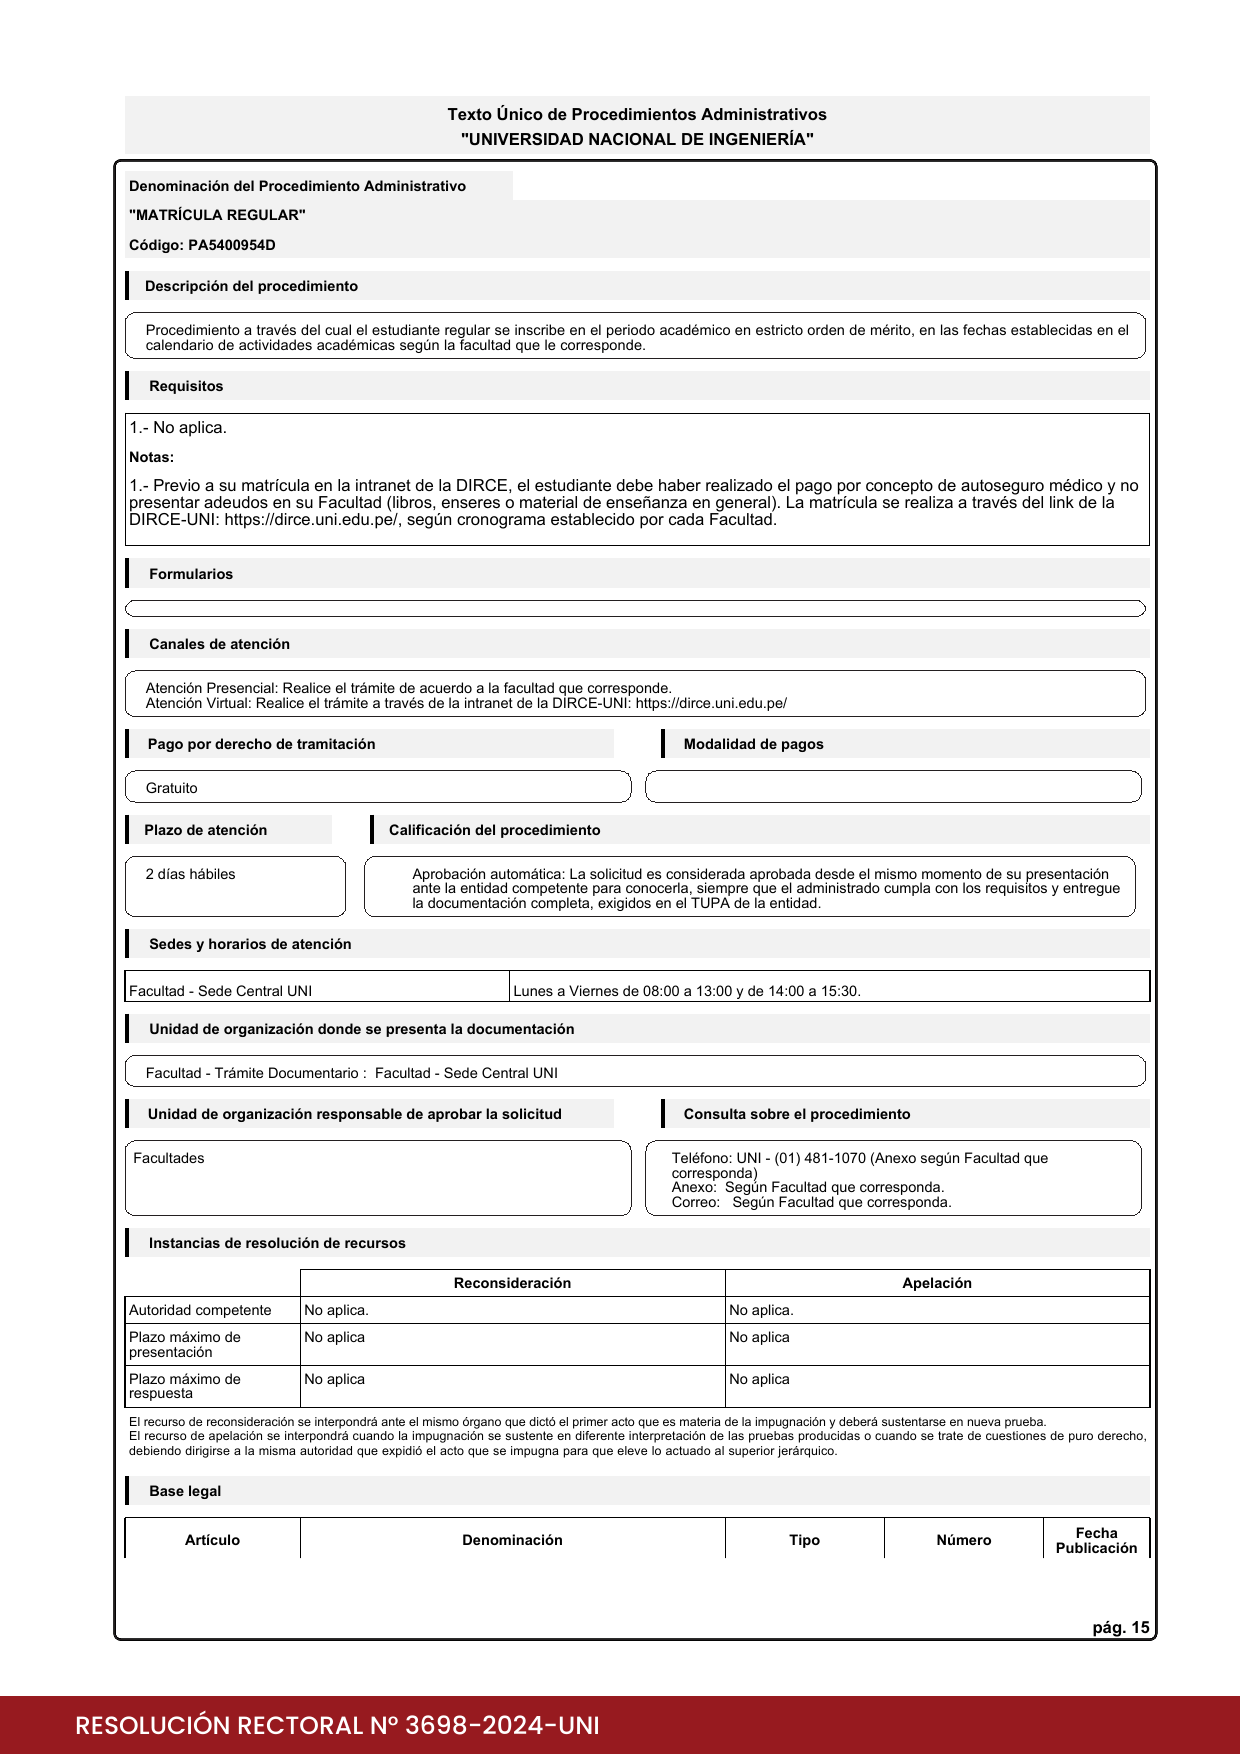
\includegraphics[width=0.85\textwidth]{evidencia_subproceso_3b_tupa_pa5400954d.png}
    \caption{Evidencia 1: Ficha del procedimiento de Matrícula Regular en el TUPA (PA5400954D, RR. N.\textsuperscript{o} 3698-2024)}
    \label{fig:evidencia_3b_tupa}
\end{figure}

\begin{figure}[H]
    \centering
    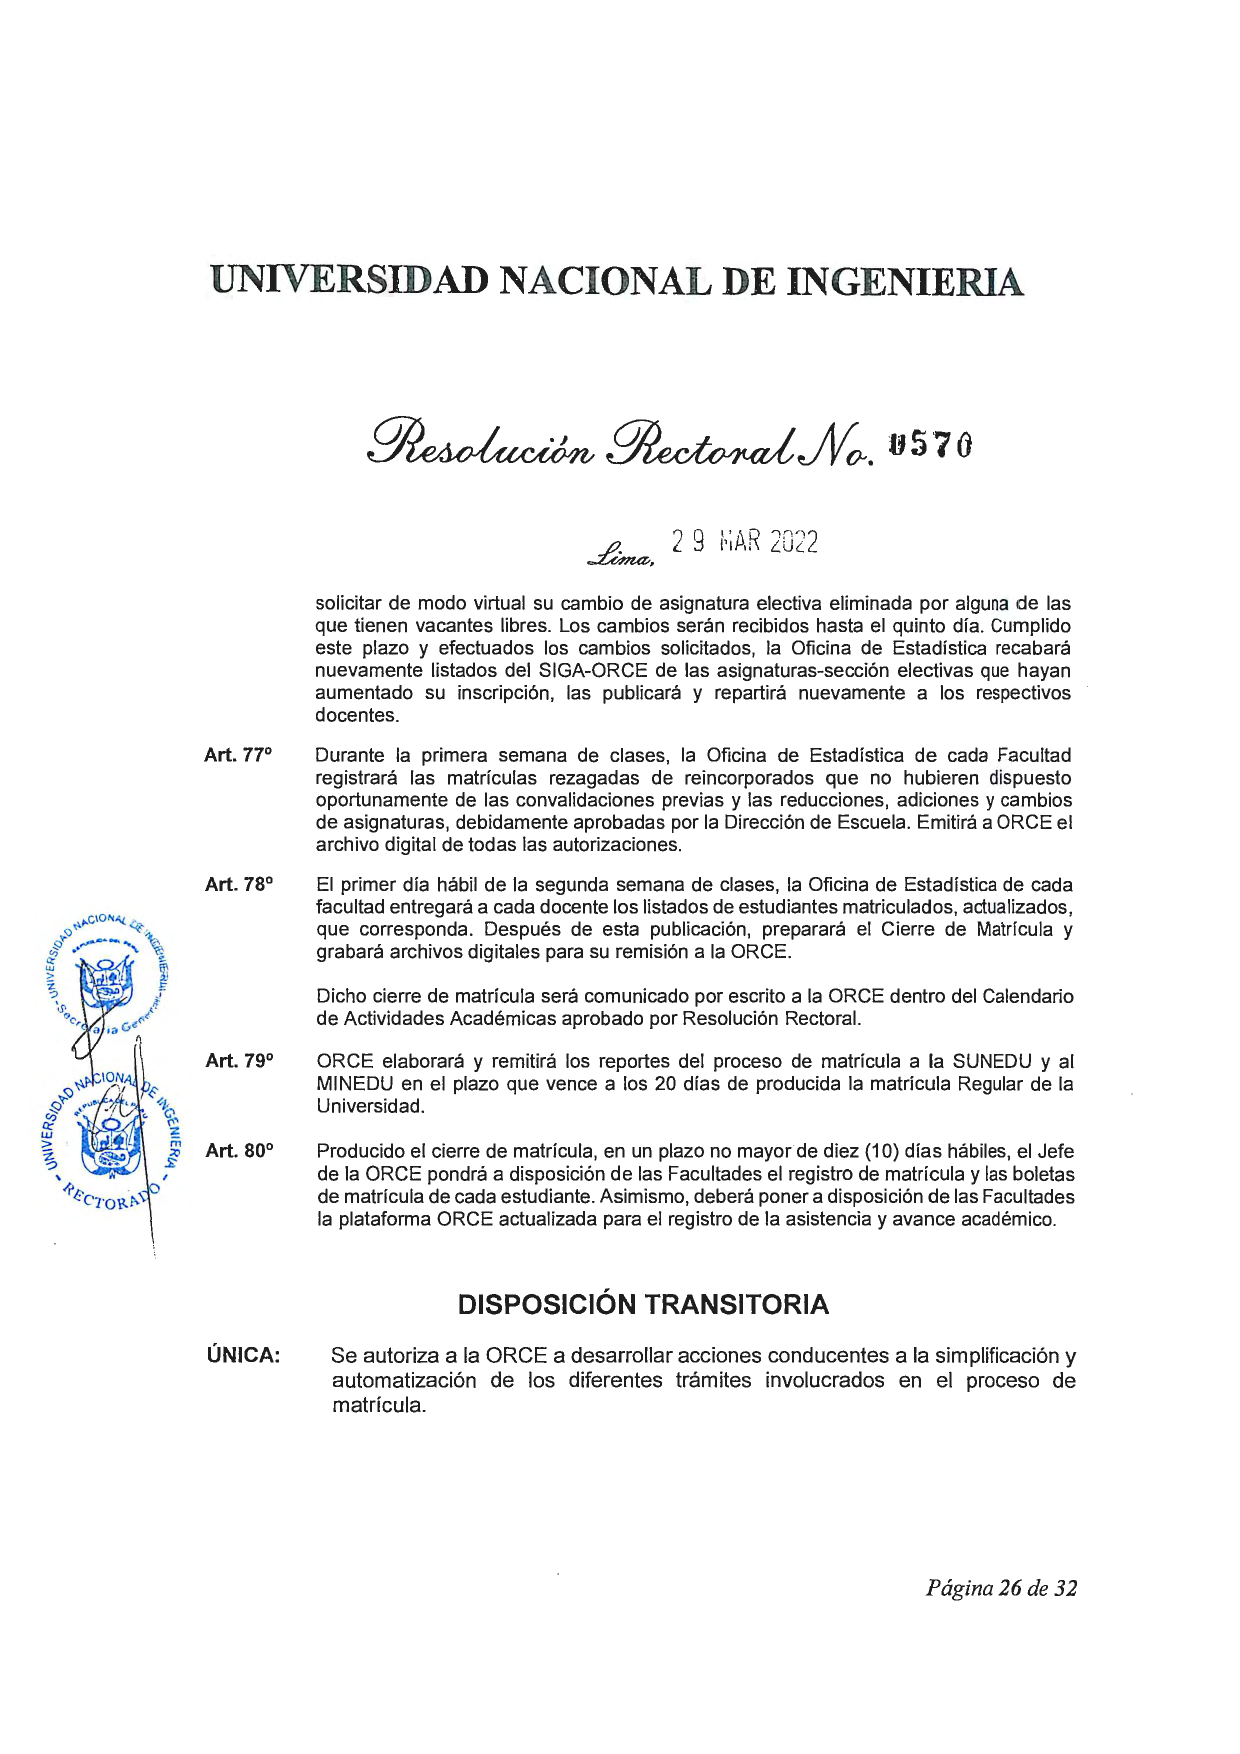
\includegraphics[width=0.85\textwidth]{evidencia_subproceso_3b_reglamento_arts77-80.png}
    \caption{Evidencia 2: Artículos 77\textdegree{}, 78\textdegree{}, 79\textdegree{} y 80\textdegree{} del Reglamento de Matrícula (RR. N.\textsuperscript{o} 570-2022)}
    \label{fig:evidencia_3b_reglamento}
\end{figure}

Además, el análisis de esta etapa se apoya en los apuntes de campo del ciclo 2026-2 tomados por un integrante del equipo, donde se registraron el aviso de cierre que envía la Facultad a la DIRCE y la falta de permisos de la Facultad para hacer cambios directos en el sistema. Al tratarse de notas de trabajo del equipo, esta información se mantiene como registro escrito interno.
